\documentclass[floatsintext,man]{apa6}

\usepackage{amssymb,amsmath}
\usepackage{ifxetex,ifluatex}
\usepackage{fixltx2e} % provides \textsubscript
\ifnum 0\ifxetex 1\fi\ifluatex 1\fi=0 % if pdftex
  \usepackage[T1]{fontenc}
  \usepackage[utf8]{inputenc}
\else % if luatex or xelatex
  \ifxetex
    \usepackage{mathspec}
    \usepackage{xltxtra,xunicode}
  \else
    \usepackage{fontspec}
  \fi
  \defaultfontfeatures{Mapping=tex-text,Scale=MatchLowercase}
  \newcommand{\euro}{€}
\fi
% use upquote if available, for straight quotes in verbatim environments
\IfFileExists{upquote.sty}{\usepackage{upquote}}{}
% use microtype if available
\IfFileExists{microtype.sty}{\usepackage{microtype}}{}

% Table formatting
\usepackage{longtable, booktabs}
\usepackage{lscape}
% \usepackage[counterclockwise]{rotating}   % Landscape page setup for large tables
\usepackage{multirow}		% Table styling
\usepackage{tabularx}		% Control Column width
\usepackage[flushleft]{threeparttable}	% Allows for three part tables with a specified notes section
\usepackage{threeparttablex}            % Lets threeparttable work with longtable

% Create new environments so endfloat can handle them
% \newenvironment{ltable}
%   {\begin{landscape}\begin{center}\begin{threeparttable}}
%   {\end{threeparttable}\end{center}\end{landscape}}

\newenvironment{lltable}
  {\begin{landscape}\begin{center}\begin{ThreePartTable}}
  {\end{ThreePartTable}\end{center}\end{landscape}}




% The following enables adjusting longtable caption width to table width
% Solution found at http://golatex.de/longtable-mit-caption-so-breit-wie-die-tabelle-t15767.html
\makeatletter
\newcommand\LastLTentrywidth{1em}
\newlength\longtablewidth
\setlength{\longtablewidth}{1in}
\newcommand\getlongtablewidth{%
 \begingroup
  \ifcsname LT@\roman{LT@tables}\endcsname
  \global\longtablewidth=0pt
  \renewcommand\LT@entry[2]{\global\advance\longtablewidth by ##2\relax\gdef\LastLTentrywidth{##2}}%
  \@nameuse{LT@\roman{LT@tables}}%
  \fi
\endgroup}


  \usepackage{graphicx}
  \makeatletter
  \def\maxwidth{\ifdim\Gin@nat@width>\linewidth\linewidth\else\Gin@nat@width\fi}
  \def\maxheight{\ifdim\Gin@nat@height>\textheight\textheight\else\Gin@nat@height\fi}
  \makeatother
  % Scale images if necessary, so that they will not overflow the page
  % margins by default, and it is still possible to overwrite the defaults
  % using explicit options in \includegraphics[width, height, ...]{}
  \setkeys{Gin}{width=\maxwidth,height=\maxheight,keepaspectratio}
\ifxetex
  \usepackage[setpagesize=false, % page size defined by xetex
              unicode=false, % unicode breaks when used with xetex
              xetex]{hyperref}
\else
  \usepackage[unicode=true]{hyperref}
\fi
\hypersetup{breaklinks=true,
            pdfauthor={},
            pdftitle={Assignment 1 : Predict 454},
            colorlinks=true,
            citecolor=blue,
            urlcolor=blue,
            linkcolor=black,
            pdfborder={0 0 0}}
\urlstyle{same}  % don't use monospace font for urls

\setlength{\parindent}{0pt}
%\setlength{\parskip}{0pt plus 0pt minus 0pt}

\setlength{\emergencystretch}{3em}  % prevent overfull lines


% Manuscript styling
\captionsetup{font=singlespacing,justification=justified}
\usepackage{csquotes}
\usepackage{upgreek}



\usepackage{tikz} % Variable definition to generate author note

% fix for \tightlist problem in pandoc 1.14
\providecommand{\tightlist}{%
  \setlength{\itemsep}{0pt}\setlength{\parskip}{0pt}}

% Essential manuscript parts
  \title{Assignment 1 : Predict 454}

  \shorttitle{Oct 14 2018}


  \author{Rahul Sangole\textsuperscript{1}}

  % \def\affdep{{""}}%
  % \def\affcity{{""}}%

  \affiliation{
    \vspace{0.5cm}
          \textsuperscript{1} Northwestern University  }



  



  \raggedbottom
  \usepackage{setspace}
  \AtBeginEnvironment{tabular}{\singlespacing}
  \AtBeginEnvironment{lltable}{\singlespacing}

\usepackage{amsthm}
\newtheorem{theorem}{Theorem}[section]
\newtheorem{lemma}{Lemma}[section]
\theoremstyle{definition}
\newtheorem{definition}{Definition}[section]
\newtheorem{corollary}{Corollary}[section]
\newtheorem{proposition}{Proposition}[section]
\theoremstyle{definition}
\newtheorem{example}{Example}[section]
\theoremstyle{definition}
\newtheorem{exercise}{Exercise}[section]
\theoremstyle{remark}
\newtheorem*{remark}{Remark}
\newtheorem*{solution}{Solution}
\begin{document}

\maketitle

\setcounter{secnumdepth}{0}



\section{Overview of Methodology}\label{overview-of-methodology}

The approach used for this assignment, modeling the \enquote{Two month's
Salary} dataset is as follows:

\begin{enumerate}
\def\labelenumi{\arabic{enumi}.}
\tightlist
\item
  Data are split into train and test datasets before further consumption
\item
  Exploratory Data Analysis (EDA) was conducted at a univariate,
  bivariate and multivariate level using numerical and graphical
  summarizations
\item
  The EDA influenced the data preparation stage in terms of transforming
  the response variable, and adding new features to the predictor matrix
\item
  Models are built on two sets of data preparation: (i) with no
  interaction terms, and (ii) with interaction terms. The types of
  models investigated are linear regressions, variable selection
  procedures on regression (best subsets, forward \& backward selection,
  lasso \& ridge), tree models (recursive partition trees \& conditional
  inference trees) and random forest models
\item
  Two staged of model building are conducted. In the first stage, models
  are built using individual R commands using each model's respective
  package (for example, \texttt{lm}, \texttt{regsubsets}, \texttt{party}
  and \texttt{partyKit} etc). This allowed a deep dive into the
  residuals and diagnostics for each model, which influenced the
  modeling strategy. Once the strategy is finalized, the \texttt{caret}
  package is used to build all models again using the
  \texttt{caret::train} interface. \texttt{caret::trainControl} is used
  to perform 10-fold cross validation to perform hyperparameter tuning
  and to determine the variation of performance for each model.
\item
  RMSE, MAE and RSquared are the metrics used to judge the performance
  of each model.
\item
  Once all the models are built using \texttt{caret}, each model is
  applied to the test dataset.
\item
  Model performance is compared on both the training and testing data,
  which reveals which model has generalized the best.
\end{enumerate}

\section{Exploratory Data Analysis}\label{exploratory-data-analysis}

\begin{figure}
\centering
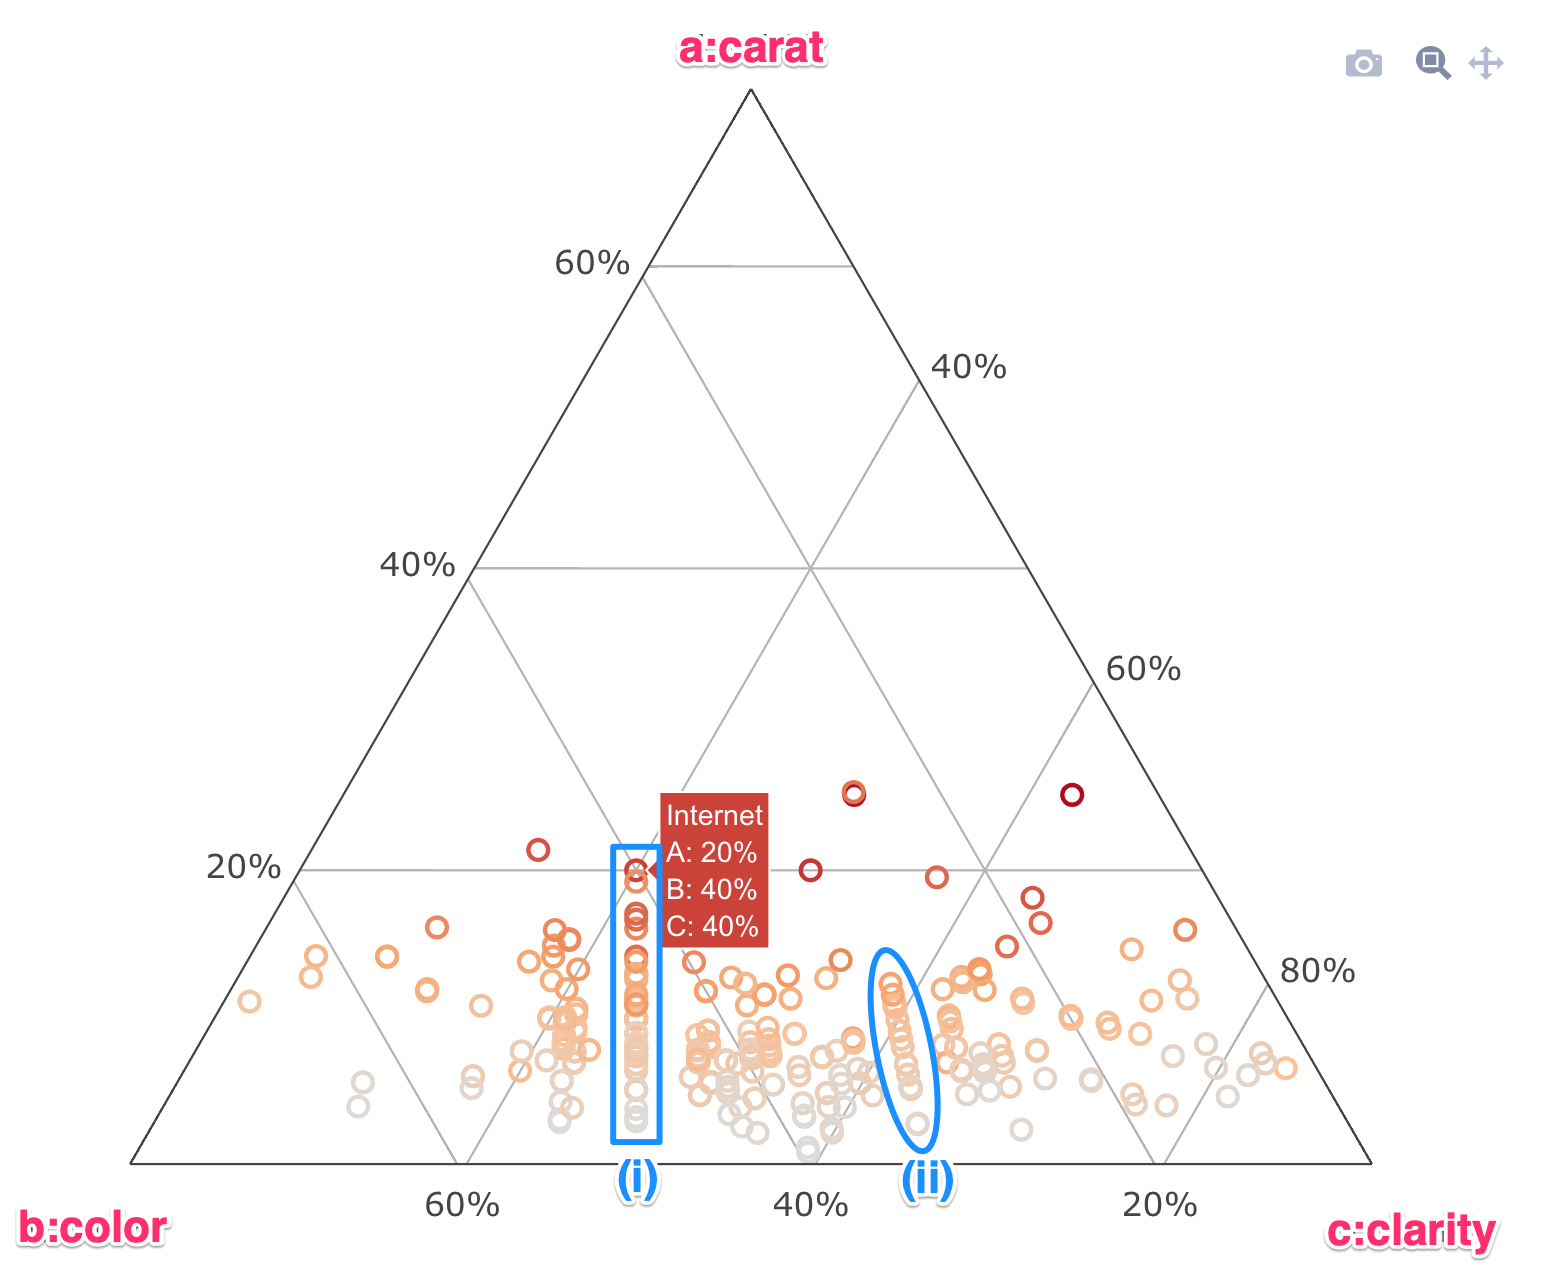
\includegraphics{../reports/ccc_ternary.png}
\caption{Ternary Plot}
\end{figure}

\begin{figure}
\centering
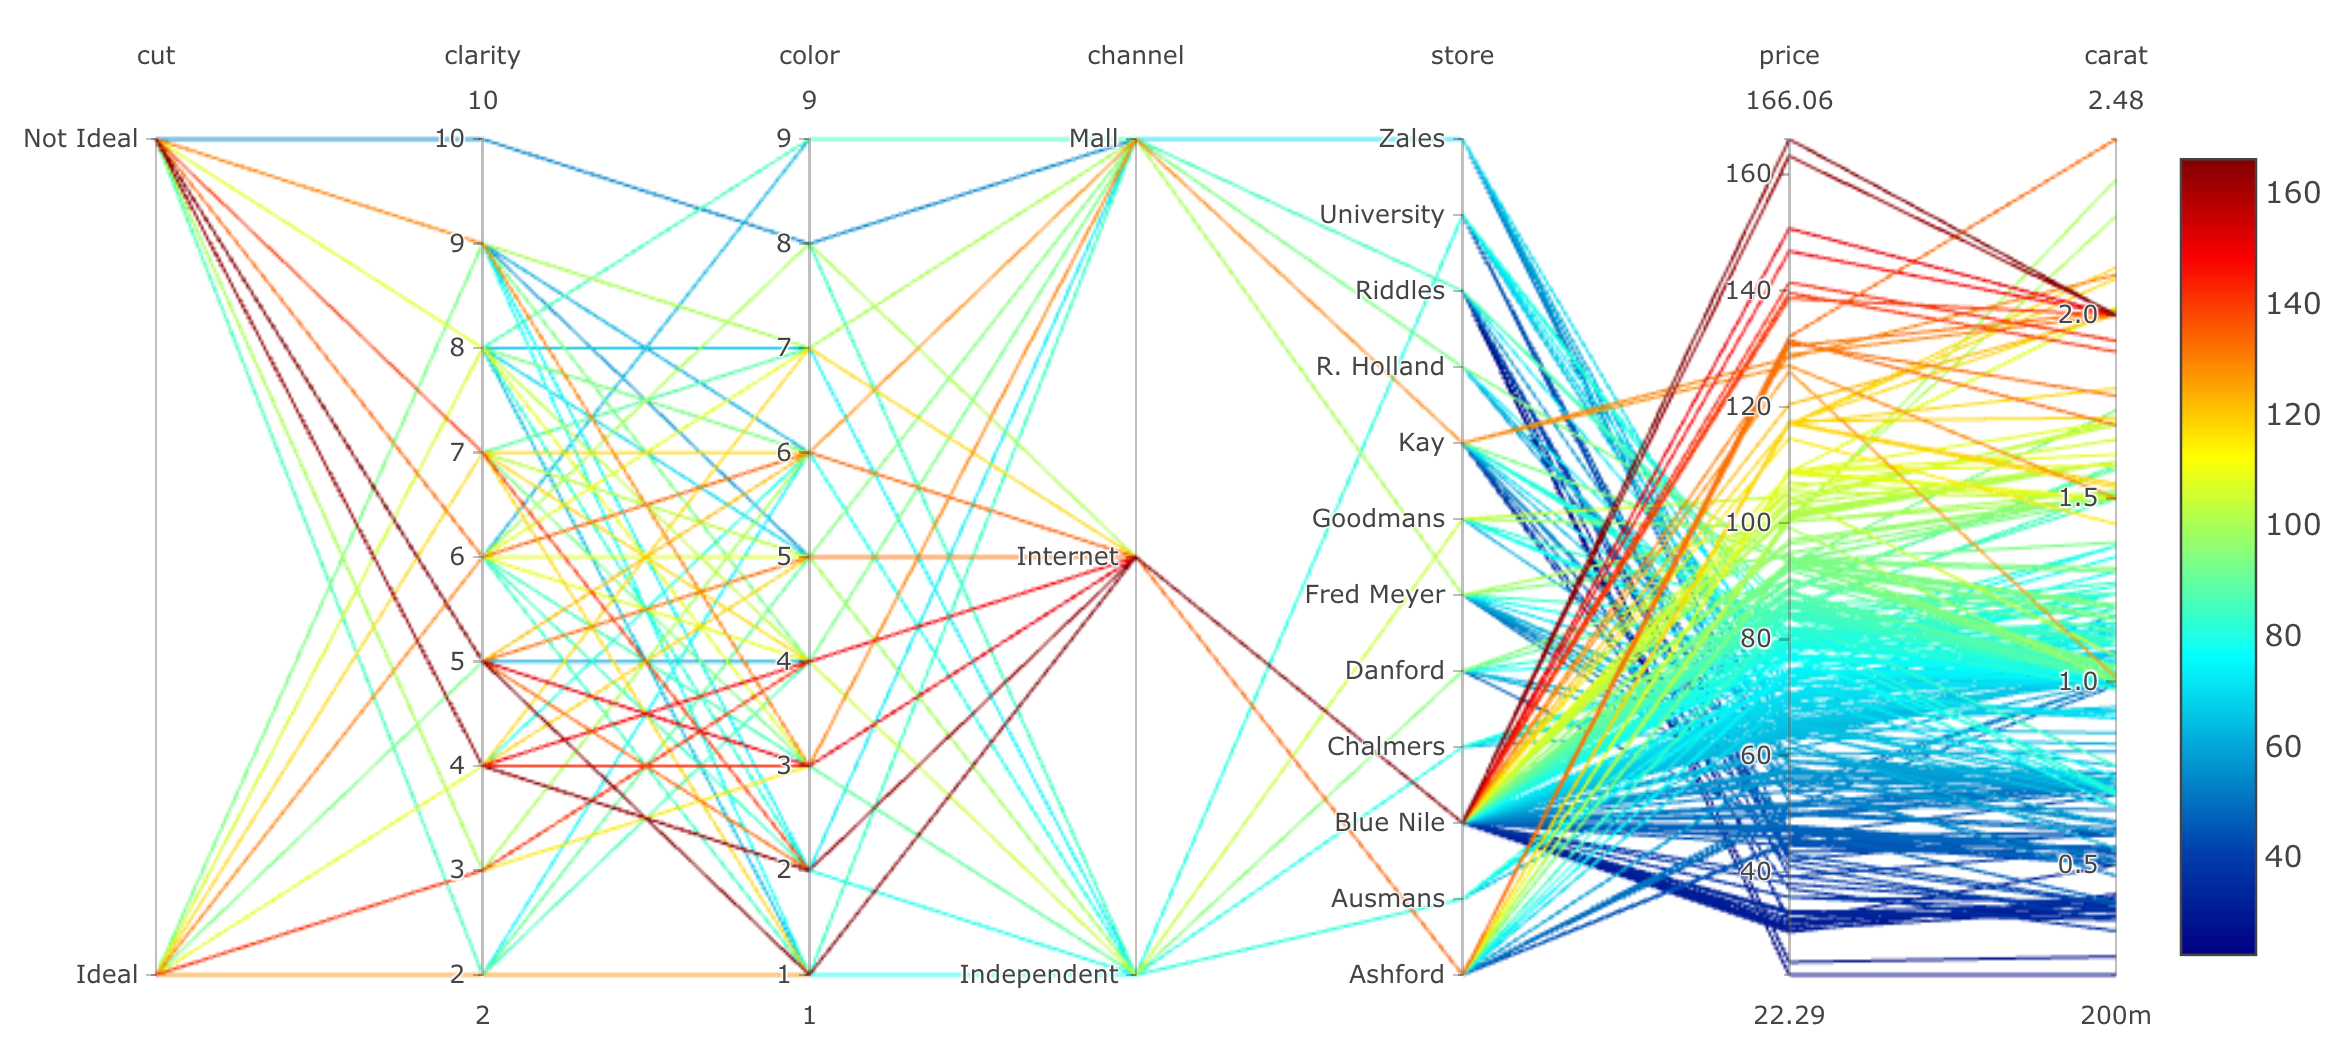
\includegraphics{../reports/parplot_1.png}
\caption{Ternary Plot}
\end{figure}

\begin{figure}
\centering
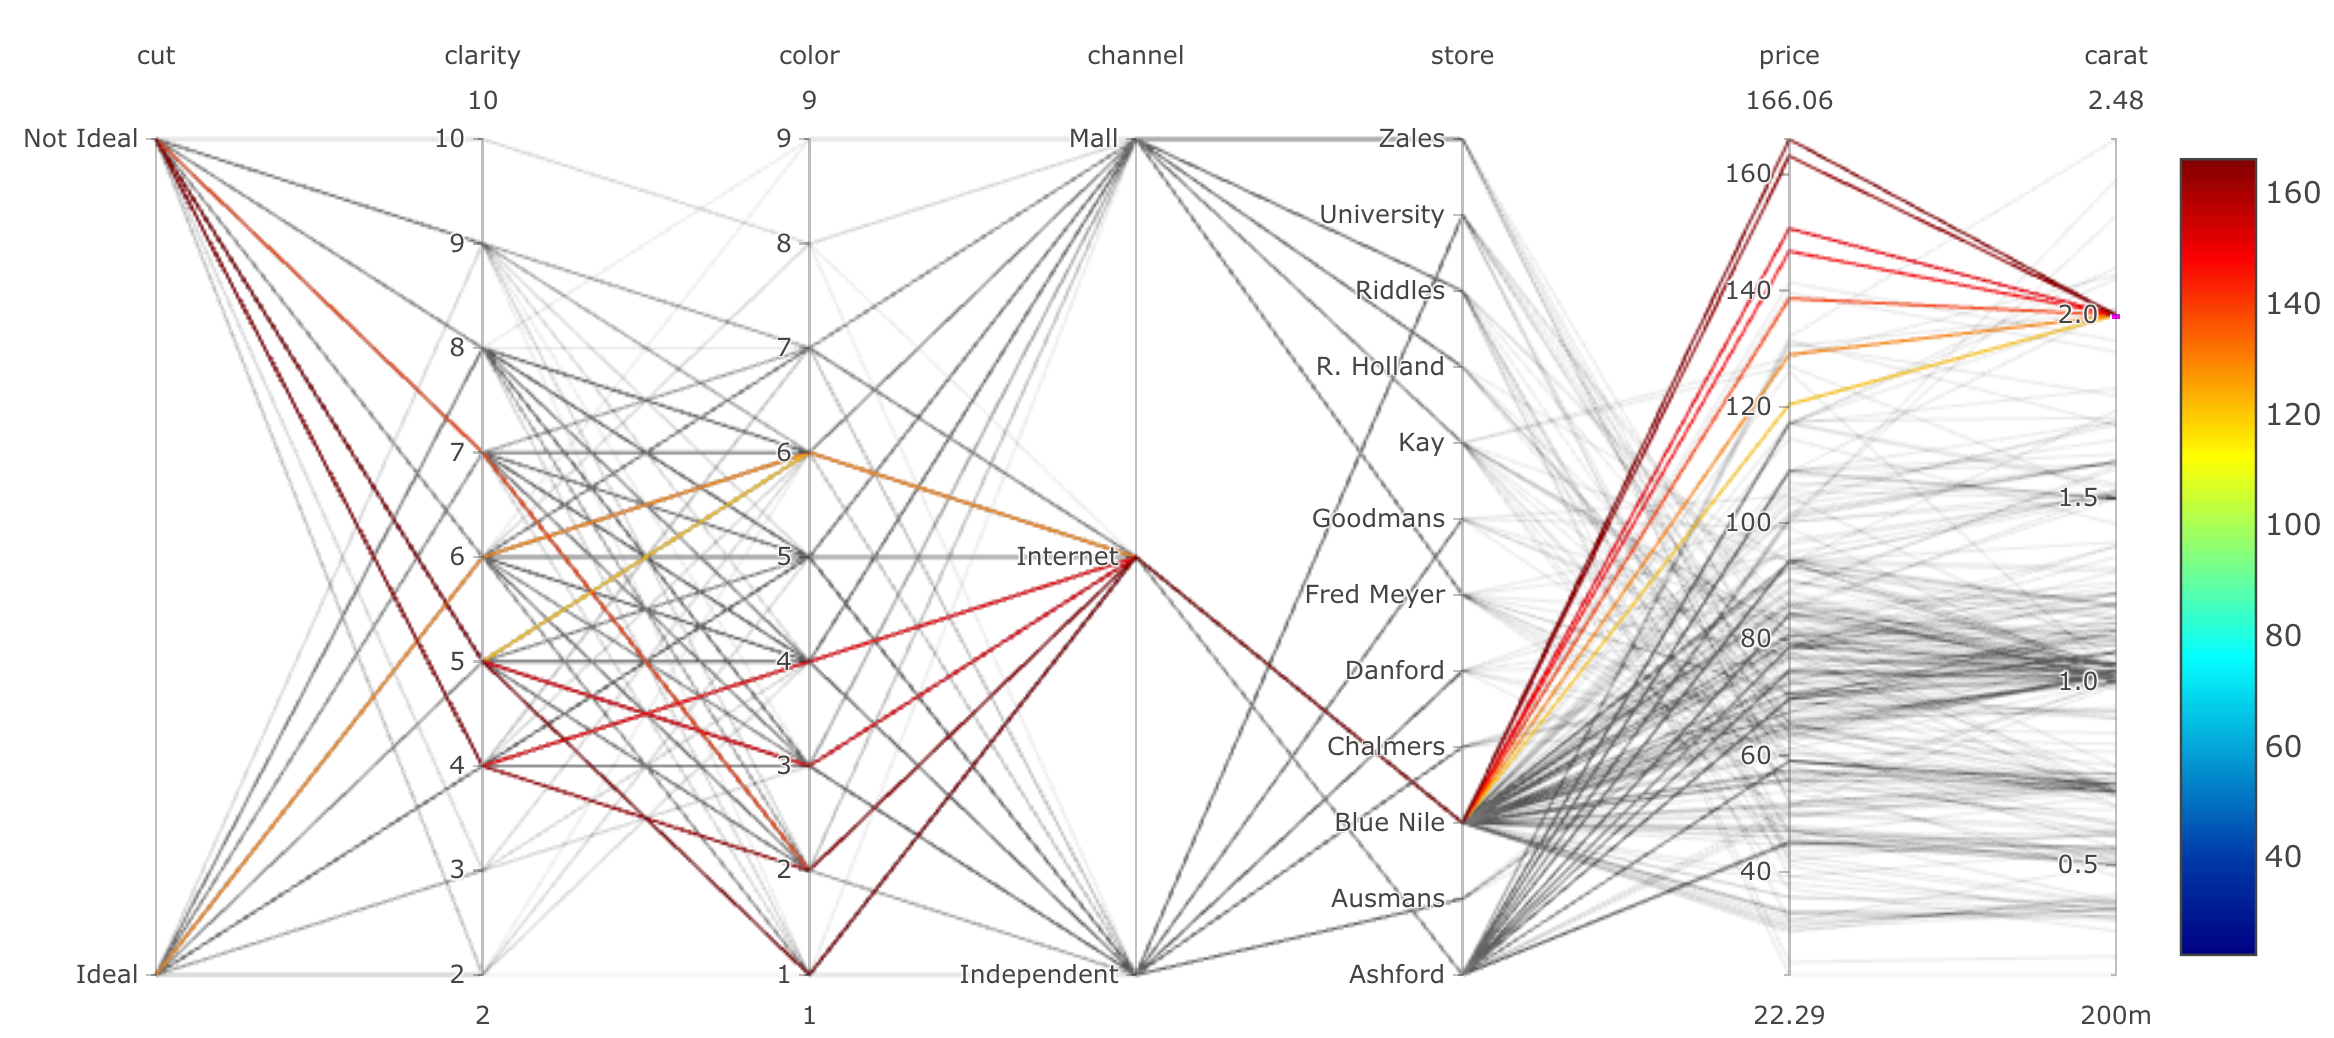
\includegraphics{../reports/parplot_3.png}
\caption{Ternary Plot}
\end{figure}

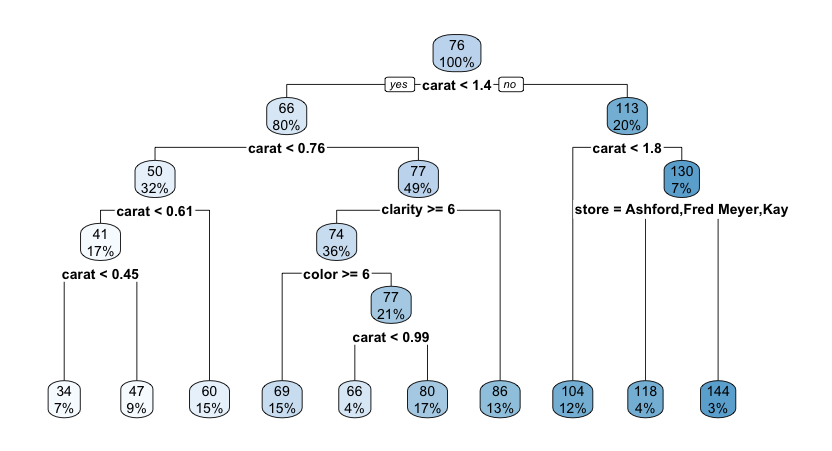
\includegraphics{../reports/rpart_tree_1way.png}
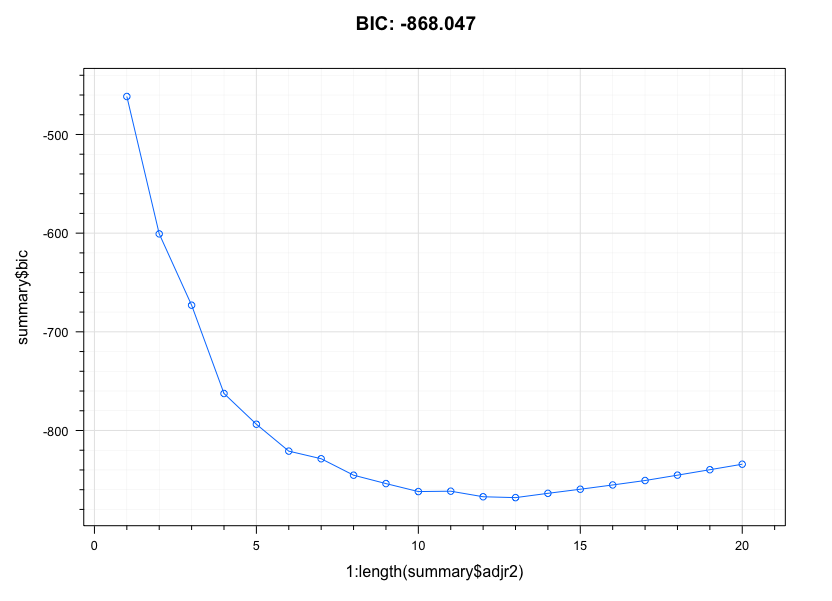
\includegraphics{../reports/bsr_bic_xy.png}
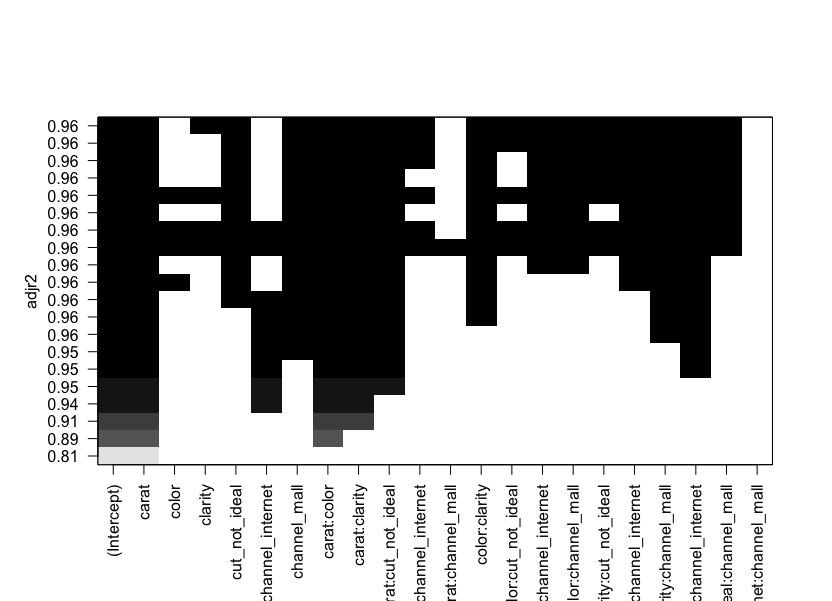
\includegraphics{../reports/bsr_lvl_r2.png}
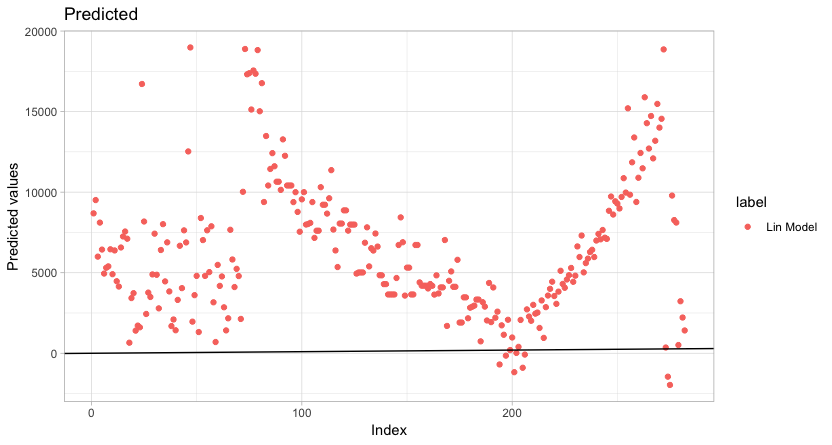
\includegraphics{../reports/lm_unsorted_yhats.png}
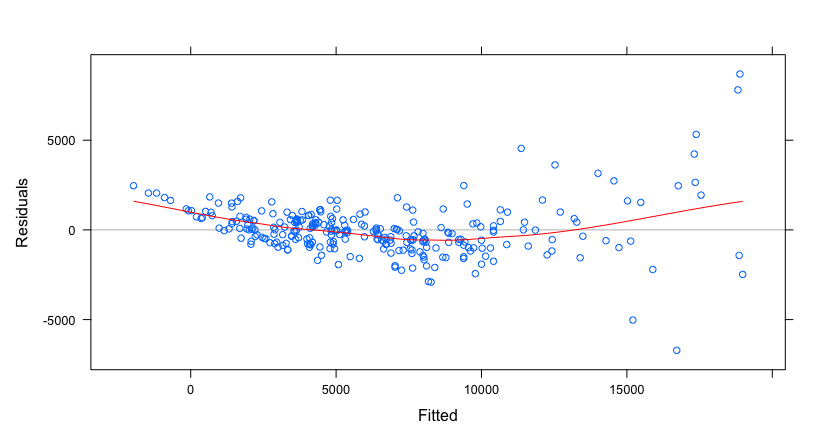
\includegraphics{../reports/lm_unsorted_residuals.png}

\section{Data Preparation}\label{data-preparation}

\section{Modeling}\label{modeling}

\section{Comparison}\label{comparison}

\section{Challenges and learnings}\label{challenges-and-learnings}

\newpage

\section{R Packages Used}\label{r-packages-used}

\newpage

\begingroup
\setlength{\parindent}{-0.5in} \setlength{\leftskip}{0.5in}

\hypertarget{refs}{}

\endgroup






\end{document}
